\documentclass[border=10pt]{standalone}
\usepackage{tikz}
\usetikzlibrary{arrows.meta,decorations.markings,patterns,calc}
\usepackage{amsmath}

\begin{document}
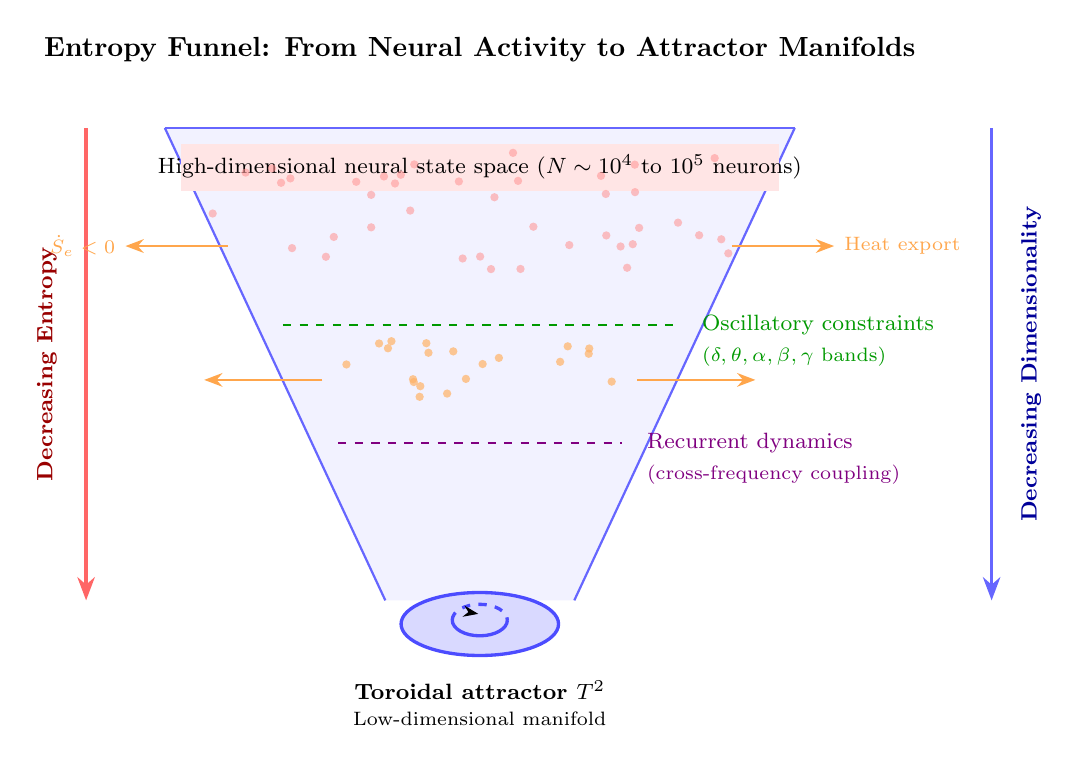
\begin{tikzpicture}[>=Stealth, font=\small]

% Funnel shape
\fill[blue!5] (-4,6) -- (-1.2,0) -- (1.2,0) -- (4,6) -- cycle;
\draw[thick, blue!60] (-4,6) -- (-1.2,0);
\draw[thick, blue!60] (4,6) -- (1.2,0);

% Top: high-dimensional activity
\draw[thick, blue!60] (-4,6) -- (4,6);
\fill[red!10] (-3.8,5.8) rectangle (3.8,5.2);
\node[font=\footnotesize] at (0,5.5) {High-dimensional neural state space ($N \sim 10^4$ to $10^5$ neurons)};

% Scattered dots at top (noisy activity)
\foreach \i in {1,...,40} {
  \pgfmathsetmacro{\rx}{-3.5 + 7*rnd}
  \pgfmathsetmacro{\ry}{4.2 + 1.5*rnd}
  \fill[red!40, opacity=0.6] (\rx,\ry) circle (1.5pt);
}

% Middle layer: oscillatory constraints
\draw[thick, dashed, green!60!black] (-2.5,3.5) -- (2.5,3.5);
\node[right, font=\footnotesize, green!60!black] at (2.7,3.5) {Oscillatory constraints};
\node[right, font=\scriptsize, green!60!black] at (2.7,3.1) {($\delta, \theta, \alpha, \beta, \gamma$ bands)};

% Partially organized dots in middle
\foreach \i in {1,...,20} {
  \pgfmathsetmacro{\rx}{-1.8 + 3.6*rnd}
  \pgfmathsetmacro{\ry}{2.5 + 0.8*rnd}
  \fill[orange!60, opacity=0.7] (\rx,\ry) circle (1.5pt);
}

% Lower layer: recurrent dynamics
\draw[thick, dashed, violet] (-1.8,2.0) -- (1.8,2.0);
\node[right, font=\footnotesize, violet] at (2.0,2.0) {Recurrent dynamics};
\node[right, font=\scriptsize, violet] at (2.0,1.6) {(cross-frequency coupling)};

% Bottom: toroidal attractor
\begin{scope}[shift={(0,-0.3)}]
  % Simple torus representation
  \draw[very thick, blue!70, fill=blue!15] (0,0) ellipse (1.0 and 0.4);
  \draw[very thick, blue!70] (-0.35,0.05) arc (180:360:0.35 and 0.2);
  \draw[very thick, blue!70, dashed] (-0.35,0.05) arc (180:0:0.35 and 0.2);
  % Trajectory on torus
  \draw[thick, red!80, decorate, decoration={markings, mark=at position 0.5 with {\arrow{>}}}] 
    (-0.8,0.1) .. controls (-0.3,0.35) and (0.3,-0.1) .. (0.8,0.15);
  \node[below, font=\footnotesize\bfseries] at (0,-0.6) {Toroidal attractor $T^2$};
  \node[below, font=\scriptsize] at (0,-1.0) {Low-dimensional manifold};
\end{scope}

% Entropy arrow on the left
\draw[<-, very thick, red!60] (-5.0,0) -- (-5.0,6);
\node[rotate=90, font=\footnotesize\bfseries, red!60!black] at (-5.5,3) {Decreasing Entropy};

% Dimensionality arrow on the right
\draw[<-, very thick, blue!60] (6.5,0) -- (6.5,6);
\node[rotate=90, font=\footnotesize\bfseries, blue!60!black] at (7.0,3) {Decreasing Dimensionality};

% Entropy export arrows
\draw[->, thick, orange!70] (-3.2,4.5) -- (-4.5,4.5) node[left, font=\scriptsize] {$\dot{S}_e < 0$};
\draw[->, thick, orange!70] (3.2,4.5) -- (4.5,4.5) node[right, font=\scriptsize] {Heat export};
\draw[->, thick, orange!70] (-2.0,2.8) -- (-3.5,2.8);
\draw[->, thick, orange!70] (2.0,2.8) -- (3.5,2.8);

% Title
\node[font=\normalsize\bfseries] at (0,7) {Entropy Funnel: From Neural Activity to Attractor Manifolds};

\end{tikzpicture}
\end{document}
